\newcommand{\clone}{\mathsf C}
\newcommand{\clonereg}{\mathsf C^{\mathrm{reg}}}
\newcommand{\rank}[1]{\mathrm{rank}(#1)}
\newcommand{\diva}{{\sc{(da)}}}
\newcommand{\homf}{{\sc{(hf)}}}
\newcommand{\fing}{{\sc{(fg)}}}
\newcommand{\eqdef}{\stackrel{\text{\tiny def}}=}
\newcommand{\trees}{{\mathsf{trees}}}
\newcommand{\terms}[1]{{\mathsf T}\!_{#1}}
\newcommand{\powerset}{{\mathsf P}}
\newcommand{\muddles}{{\mathsf M}}
\newcommand{\unit}{\mathsf{unit}}
\newcommand{\flatt}{\mathsf{flat}}
\newcommand{\aalg}{\ensuremath{\mathbf{A}}\xspace}
\newcommand{\balg}{\ensuremath{\mathbf{B}}\xspace}
\newcommand{\Nat}{\mathbb N}
\newcommand{\hsp}{{\sc hsp \xspace}}
\newcommand{\mso}{{\sc mso}\xspace}
\newcommand{\msoone}{{\sc mso$_1$ \xspace}}
\newcommand{\msotwo}{{\sc mso$_2$ \xspace}}

\newcommand{\hs}{{\sc hs \xspace}}
\newcommand{\aut}{\mathcal A}
\newcommand{\nodes}{\mathsf{nodes}}
\newcommand{\set}[1]{\{#1\}}
\newcommand{\dom}{\mathsf{dom}}
%\newcommand{\ker}{\mathsf{ker}}
\newcommand{\game}{\mathsf G}
\newcommand{\mult}{\mathsf{mult}}
\newcommand{\parfun}{\rightharpoonup}
\newcommand{\monad}{\mathsf M}
\newcommand{\facto}{\mathsf F}
\newcommand{\poly}[2]{\mathsf{pol}_{#1}#2}

%
%%Janusz%%
\newcommand{\ens}[1]{{\ensuremath{#1}}\xspace}
%Strzałki
\newcommand{\ra}{\rightarrow}
\newcommand{\xra}[1]{\xrightarrow{#1}}
\newcommand{\Z}{\ensuremath{\mathbb{Z}}\xspace}
\DeclareMathOperator{\join}{fuse}
\DeclareMathOperator{\forget}{forget}
\DeclareMathOperator{\sources}{sources}
\DeclareMathOperator{\cyclic}{cycle}
\DeclareMathOperator{\charact}{char}%komenda \char jest już defined
\newcommand{\allv}[1]{\ensuremath{\sources(#1) \cup \{\bullet\}}\xspace} %"allv = all vertices", czyli source'y plus \bullet
\newcommand{\Registers}{\ensuremath{\mathcal{R}}\xspace}
\newcommand{\enum}[3]{#1_{#2}, \ldots, #1_{#3}}
\newcommand{\iffdef}{\stackrel{def}{\Leftrightarrow}}
\newcommand{\N}{\ens{\mathbb{N}}}
\newcommand{\Q}{\ens{\mathbb{Q}}}
\newcommand{\Cc}{\ensuremath{\mathcal{C}}\xspace}
\def\sizemacierzy{0.4cm}
\def\GaSize{\large}
\def\ZeroSize{\Large}
\def\GprimSize{\Large}
\def\HprimSize{\LARGE}
\newlength{\picPrzesuniecie}
\setlength{\picPrzesuniecie}{4.5cm}
\def\skalamatadjacency{0.8}
\def\skalamacierzy{1}
\newcommand{\primecofact}[2]{\overline{#1}^{#2}}%definicja phi dla wielomianu charakterystycznego -- pierwszy komponent, argumenty #1 = graf, #2 = nazwa source'a względem którego sklejamy
\newcommand{\rest}[2]{\widetilde{#1}^{#2}}%definicja phi dla wielomianu charakterystycznego -- drugi komponent, argumenty #1 = graf, #2 = nazwa source'a względem którego sklejamy
\newcommand{\algcyclic}{\ensuremath{\mathbf{C}}\xspace}
\newcommand{\algebradefinitionwithhfill}[2]%argumenty to: Uniwersum i Operacje
{
	{
		\begin{description}
			\item[Domain:] \hfill \\ #1
			\item[Basic operations:] \hfill \\ #2
		\end{description}
	}
}
\newcommand{\algebradefinition}[2]%argumenty to: Uniwersum i Operacje
{
	{
		\begin{description}
			\item[Domain:]  #1
			\item[Basic operations:]  #2
		\end{description}
	}
}
\newcommand{\op}{\ensuremath{\tau}\xspace}
%register transducers
\def\valu{\mathbf{v}}
\DeclareMathOperator{\out}{output}
\newcommand{\qinit}{\ensuremath{q_{init}}\xspace}
\newcommand{\initval}{\ensuremath{{\mathbf{t}_0}}\xspace}

%Hilbert Method
%
\newcommand{\simby}{\preceq_{pol}}
%\newcommand{\Registers}{\ens{\mathcal{R}}}
\newcommand{\Transitions}{\ens{\Delta}}
\newcommand{\bt}{\ens{\mathbf{t}}}
\newcommand{\InputAlphabet}{\ens{\Sigma}}
\newcommand{\Input}{\ens{\Sigma^*}}
\newcommand{\cl}[1]{\ens{\overline{#1}}}
\newcommand{\COSq}[1]{\ens{(#1_q)_{q \in Q}}}
\newcommand{\Fq}{\COSq{F}}
\newcommand{\Iq}{\COSq{I}}
\newcommand{\Xq}{\COSq{X}}
\DeclareMathOperator{\II}{\mathcal{I}}
\DeclareMathOperator{\VV}{\mathcal{V}}
%%Janusz-koniec
%
\newcounter{ourexamplecounter}
\newenvironment{example}{
\medskip

\refstepcounter{ourexamplecounter}
\smallskip\noindent{\textbf{{Example \arabic{ourexamplecounter}. }}}}{
$\Box$ \smallskip 
}

\newcounter{runningcounter}
\newenvironment{running}{
\medskip

\refstepcounter{runningcounter}
\smallskip\noindent{\textbf{{Running Example \arabic{runningcounter}. }}}}{
$\Box$ \smallskip 
}




\newcommand{\mypic}[1]{
	\begin{center}
		\includegraphics[page=#1,scale=0.4]{pics}
	\end{center}
}

\newcommand{\treewidthtotreewidth}[2]{treewidth$_{\leqslant #1}$-to-treewidth$_{\leqslant #2}$}

\newcommand{\treetotreewidth}[1]{tree-to-treewidth$_{< #1}$\xspace}

\newcommand{\homset}{\mathrm
{Hom}}

\newcommand{\powerseries}[1]{#1 [\![x]\!]}
\newcommand{\natx}{\Nat_{0}[\![x]\!]}
% \newcommand{\powerseries}[1]{\mathbb Q [\![#1]\!]}

\newcommand{\Ring}{\ens{\mathbb K}}
\newcommand{\Field}{\mathbb F}
\newcommand{\Rat}{\mathbb Q}
\newcommand{\Int}{\mathbb Z}
\newcommand{\Real}{\mathbb R}
% \newcommand{\Nat}{\mathbb N}


\newcommand{\smallparagraph}[1]{\smallskip \noindent {\bf #1. }}

\newcommand{\Rr}{{\mathcal R}}
\newcommand{\Ss}{{\mathcal S}}
\newcommand{\Tt}{{\mathcal T}}
\newcommand{\Ff}{{\mathcal F}}
\newcommand{\myunderbrace}[2]{\underbrace{#1}_{\mathclap{\text{#2}}}}
\newcommand{\myoverbrace}[2]{\overbrace{#1}^{\mathclap{\text{#2}}}}

\newcommand{\Aa}{{\ens{\mathcal A}}}
\newcommand{\Bb}{{\mathcal B}}

\newcommand{\decisionproblem}[3]
{
	\begin{description}
		\item[Name:] #1
		\item[Instance:]  #2
		\item[Question:] #3 
	\end{description}
}
\DeclareMathOperator{\eqzeroinalgb}{\ensuremath{
		%p_{((-) =_B)}
		p_{0_B}
	}}
\newcommand{\Zrat}{\ens{\Z^{\mathrm{rat}}[\![x]\!]}}
\newcommand{\regTsover}[1]{register transducers over ${#1}$}
\newcommand{\polTsover}[1]{register transducers over ${#1}$}
\newcommand{\regTover}[1]{register transducer over ${#1}$}
\newcommand{\polTover}[1]{register transducer over ${#1}$}
\newcommand{\edgeendpoints}{\ens{\mathrm{endpoint}}}